Visualization features are strongly dependant on the imaging acquisiton process as depicted in Section \ref{sec::Workflow}.
In this step, the user performing the imaging acquistion decides whether segments are transparent or not.
\begin{figure}
  \centering
  \begin{minipage}{.5\textwidth}
    \centering
    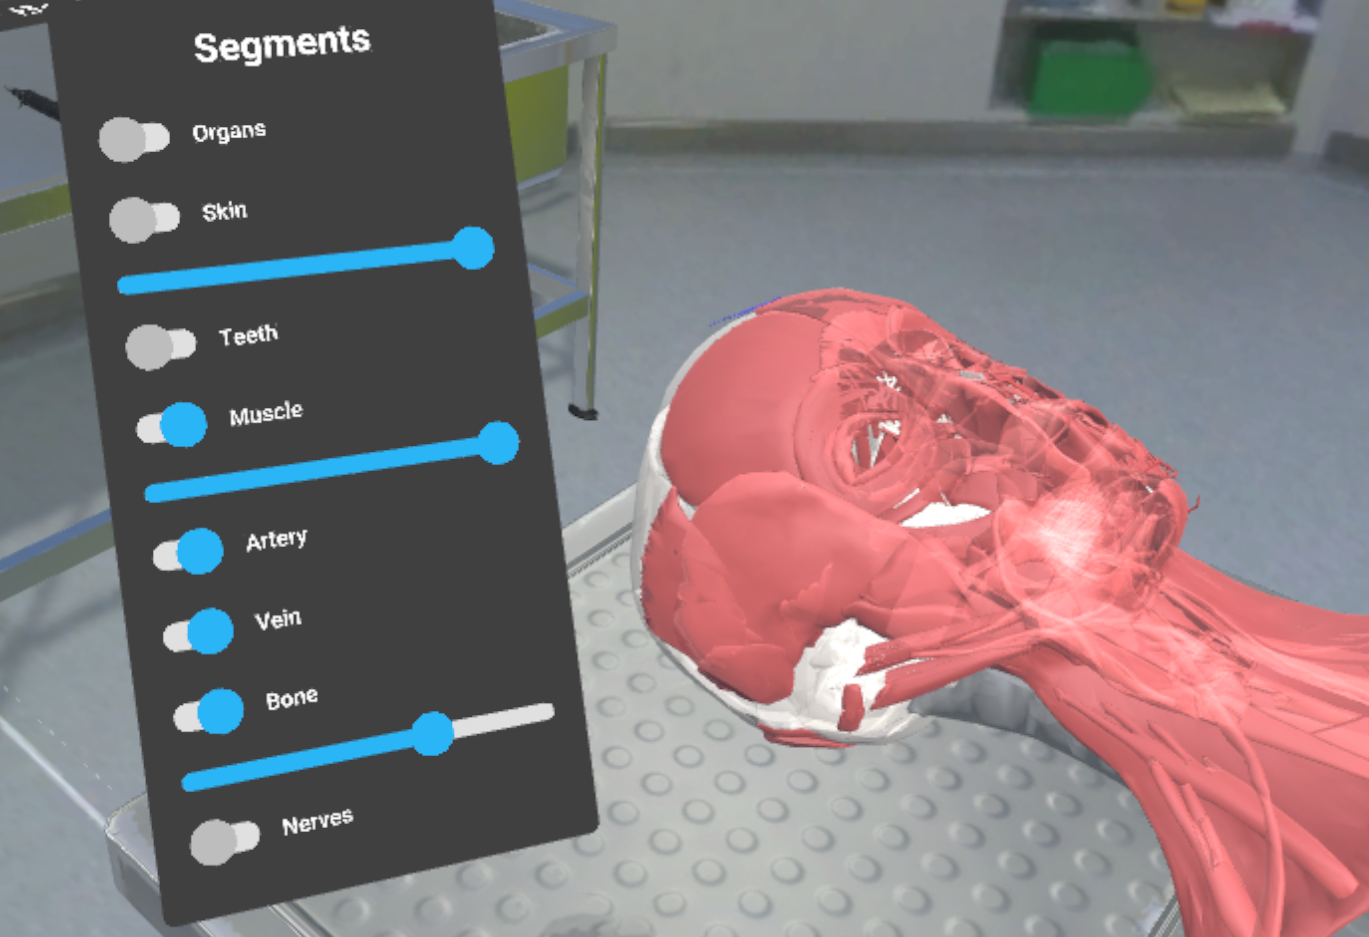
\includegraphics[width=0.95\linewidth]{images/implementation/features/visualization/segments_1.png}
  \end{minipage}%
  \begin{minipage}{.5\textwidth}
    \centering
    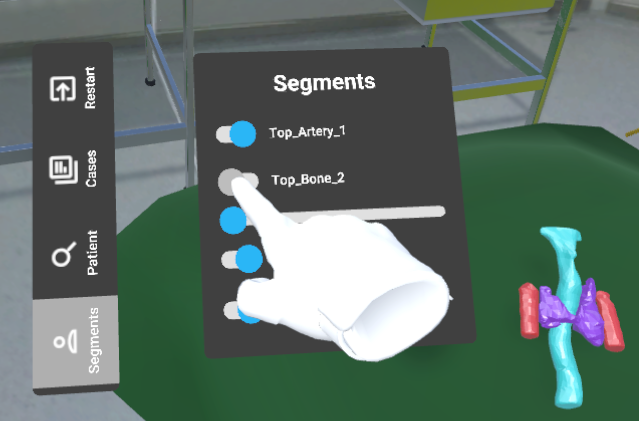
\includegraphics[width=0.95\linewidth]{images/implementation/features/visualization/segments_2.png}
  \end{minipage}
  \caption{\label{fig::Segmentation}Visualization - Segmentation}
\end{figure}

In Figure \ref{fig::Segmentation}, the process of activating and deactivating specific segments is described.
Users can also decide to adjust the transparency of segments as desired.

\begin{figure}[ht!]
    \centering
    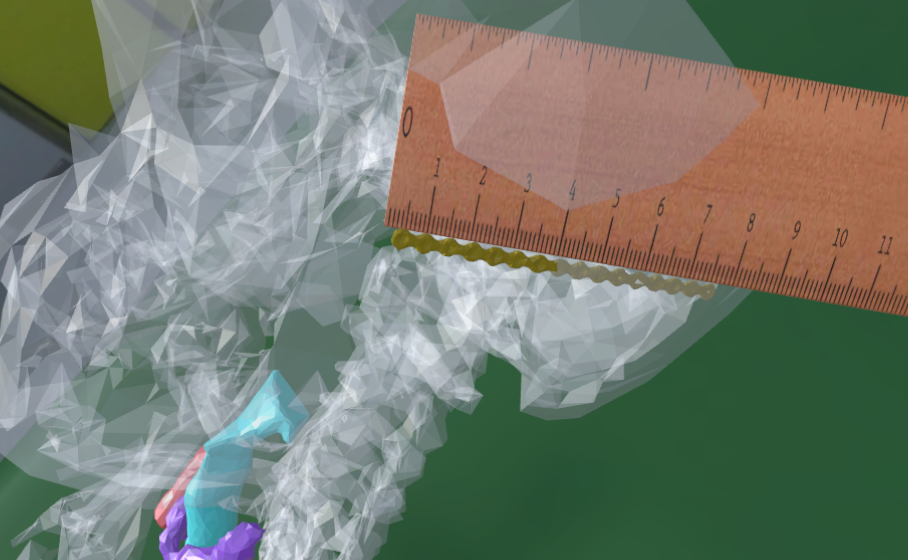
\includegraphics[width=\linewidth]{images/implementation/features/visualization/ruler.png}
    \caption{\label{fig::FeatureRuler} Ruler for Checking distances}
\end{figure}

\input{sections/4_implementation/features/visualization/explodeview.tex}